\documentclass[a4paper,12pt]{report}
\usepackage[utf8]{inputenc} % this is needed for fr umlauts
\usepackage[french]{babel} % this is needed for fr umlauts
\usepackage[T1]{fontenc}    % this is needed for correct output of umlauts in pdf
\usepackage{textcomp}
\usepackage[margin=2.5cm]{geometry} %layout
\usepackage[usenames,dvipsnames,svgnames,table]{xcolor}
\usepackage[pdftex,urlcolor=blue,pdfstartview=FitH]{hyperref}
\usepackage{hyperref}  
\usepackage{listings} 
\usepackage{graphicx}
\usepackage{subfig}
\usepackage{array}
\usepackage[section]{placeins}
\usepackage[usenames,dvipsnames,svgnames,table]{xcolor}
\usepackage[pdftex,urlcolor=blue,pdfstartview=FitH]{hyperref}

\usepackage[ %quotation package
    left = \flqq,% 
    right = \frqq,% 
    leftsub = \flqq,% 
    rightsub = \frqq%
]{dirtytalk}

\lstset{ %
  language=Java,                  % the language of the code
  basicstyle=\footnotesize,       % the size of the fonts that are used for the code
  numbers=left,                   % where to put the line-numbers
  numberstyle=\tiny\color{gray},  % the style that is used for the line-numbers
  stepnumber=1,                   % the step between two line-numbers. If it's 1, each line 
                                  % will be numbered
  numbersep=5pt,                  % how far the line-numbers are from the code
  backgroundcolor=\color{white},  % choose the background color. You must add \usepackage{color}
  showspaces=false,               % show spaces adding particular underscores
  showstringspaces=false,         % underline spaces within strings
  showtabs=false,                 % show tabs within strings adding particular underscores
  frame=single,                   % adds a frame around the code
  rulecolor=\color{black},        % if not set, the frame-color may be changed on line-breaks within not-black text (e.g. commens (green here))
  tabsize=4,                      % sets default tabsize to 2 spaces
  % captionpos=b,                   % sets the caption-position to bottom
  breaklines=true,                % sets automatic line breaking
  breakatwhitespace=false,        % sets if automatic breaks should only happen at whitespace
  title=\lstname,                 % show the filename of files included with \lstinputlisting;
                                  % also try caption instead of title
  keywordstyle=\color{blue},          % keyword style
  commentstyle=\color{olive},       % comment style
  stringstyle=\color{violet},         % string literal style
  escapeinside={\%*}{*)},            % if you want to add a comment within your code
  morekeywords={*,...}               % if you want to add more keywords to the set
}
%%%%%%%%%%%%%%%%%%%%%%%%%%%%%%%%%%%%%%%%%%%%%%%%%%%%%%%%%%%%%%%%%%%%%%
% Variablen                                                          %
%%%%%%%%%%%%%%%%%%%%%%%%%%%%%%%%%%%%%%%%%%%%%%%%%%%%%%%%%%%%%%%%%%%%%%
\newcommand{\authorName}{Pierre Labadille, Alexandre Ducreux}
\newcommand{\tags}{\authorName, Java, Thread, Socket, Swing, Chat, M2-DNR2i}
\title{Rapport de projet Java : Java Chat}
\title{%
  \begin{figure}[!ht]%
    \centering
    
\includegraphics[width=5cm]{unicaen.jpg}%
  \end{figure}%
  Rapport de projet : Java Chat \\
  \large Sujet proposé par Yann Mathet \\
  \large Université de Caen Normandie - M2-DNR2i \\
    Code visualisable sur \href{https://github.com/alimux/JavaChat}{github} ou en annexe (codeSource.pdf).
}
\author{\authorName}
\date{\today}

%%%%%%%%%%%%%%%%%%%%%%%%%%%%%%%%%%%%%%%%%%%%%%%%%%%%%%%%%%%%%%%%%%%%%%
% PDF Meta information                                               %
%%%%%%%%%%%%%%%%%%%%%%%%%%%%%%%%%%%%%%%%%%%%%%%%%%%%%%%%%%%%%%%%%%%%%%
\hypersetup{
  pdfauthor   = {\authorName},
  pdfkeywords = {\tags},
  pdftitle    = {rapportJavaChat_cc2017}
} 

%%%%%%%%%%%%%%%%%%%%%%%%%%%%%%%%%%%%%%%%%%%%%%%%%%%%%%%%%%%%%%%%%%%%%%
% USAGE MEMO                                                         %
%%%%%%%%%%%%%%%%%%%%%%%%%%%%%%%%%%%%%%%%%%%%%%%%%%%%%%%%%%%%%%%%%%%%%%
% link: \href{LINK}{TEXT}
% footnote: \footnote{CONTENT}
% quote: \say{CONTENT}
% italics: \emph{CONTENT}
% bold: \textbf{CONTENT}
% jump line \smallbreak, \midbreak, \bigbreak
% title: \chapter{NAME}, \section{NAME}, \subsection{NAME}
% list: \begin{itemize} \item CONTENT \item CONTENT \end{itemize}
% figure: \begin{figure}[!ht]% \centering \includegraphics[width=SIZEcm]{PATH}
% multi-figure: ------
% \begin{figure}[!ht]%
% \centering
% \subfloat[FIGURE_NAME]{{\includegraphics[width=SIZEcm]{PATH} }}%
% \qquad
% \subfloat[FIGURE_NAME]{{\includegraphics[width=SIZEcm]{PATH} }}%
% \caption{DATA_SET_NAME}%
% IF in SUBSECTION: \FloatBarrier
% -------------------
% code inclusion: -----
% \begin{lstlisting}[language=LANGAGE, title=FILE_NAME]
% CONTENT
% \end{lstlisting}
% -------------------
%%%%%%%%%%%%%%%%%%%%%%%%%%%%%%%%%%%%%%%%%%%%%%%%%%%%%%%%%%%%%%%%%%%%%%
%%%%%%%%%%%%%%%%%%%%%%%%%%%%%%%%%%%%%%%%%%%%%%%%%%%%%%%%%%%%%%%%%%%%%%

%%%%%%%%%%%%%%%%%%%%%%%%%%%%%%%%%%%%%%%%%%%%%%%%%%%%%%%%%%%%%%%%%%%%%%
% THE DOCUMENT BEGINS                                                %
%%%%%%%%%%%%%%%%%%%%%%%%%%%%%%%%%%%%%%%%%%%%%%%%%%%%%%%%%%%%%%%%%%%%%%
\begin{document}
  \maketitle
  \tableofcontents

  \chapter{Introduction}

    \section{Présentation du projet}
    Le but de ce projet est de proposer une application permettant à plusieurs utilisateurs de communiquer entre eux par le biais d'un serveur sur le système du "chat". En outre, les utilisateurs de ce système pourront se déplacer au drag'n'drop sur une carte et voir les autres personnes présentent ainsi que leurs localisation. Cette "carte" fait l'originalité de l'application. En effet, seul les personnes se trouvant dans un certain rayon d'écoute, représenté par un cercle, pourront voir les messages envoyés par un autre utilisateur. 
    \medbreak
    Ce projet est développé intégralement en Java en utilisant Swing et le système de socket et de thread. Le projet est découpé en deux grandes parties: le serveur qui permet de gérer l'interaction entre n utilisateurs ainsi que le client qui permet leurs permets d'avoir une interface et d'intéragir avec les autres.
    \bigbreak
    Au sujet de la répartition du travail, celle-ci a été assez simple:
    \begin{itemize}
      \item La réflexion et l'architecture de l'application a été entièrement pensée et réalisée de concert.
      \item La partie interface client (l'interaction utilisateur, l'interface client et la gestion des événements) a été réalisée par Alexandre Ducreux.
      \item La partie serveur et communication client-serveur (et inversement) a été réalisée par Pierre Labadille.
    \end{itemize}
    \medbreak
    Celà étant, il faut noter que nous avons tous les deux apportés des modifications dans toute l'application afin de mettre en place certains méchanismes. La séparation des tâches comme exprimée ci-dessus est donc plus absolue que la réalité. 

    \section{Modèle UML}
      Veuillez noter que ces deux annexes sont zoomables. Elles sont également disponibles en annexe au format png.
      \medbreak
      \begin{figure}[!ht]%
        \centering 
        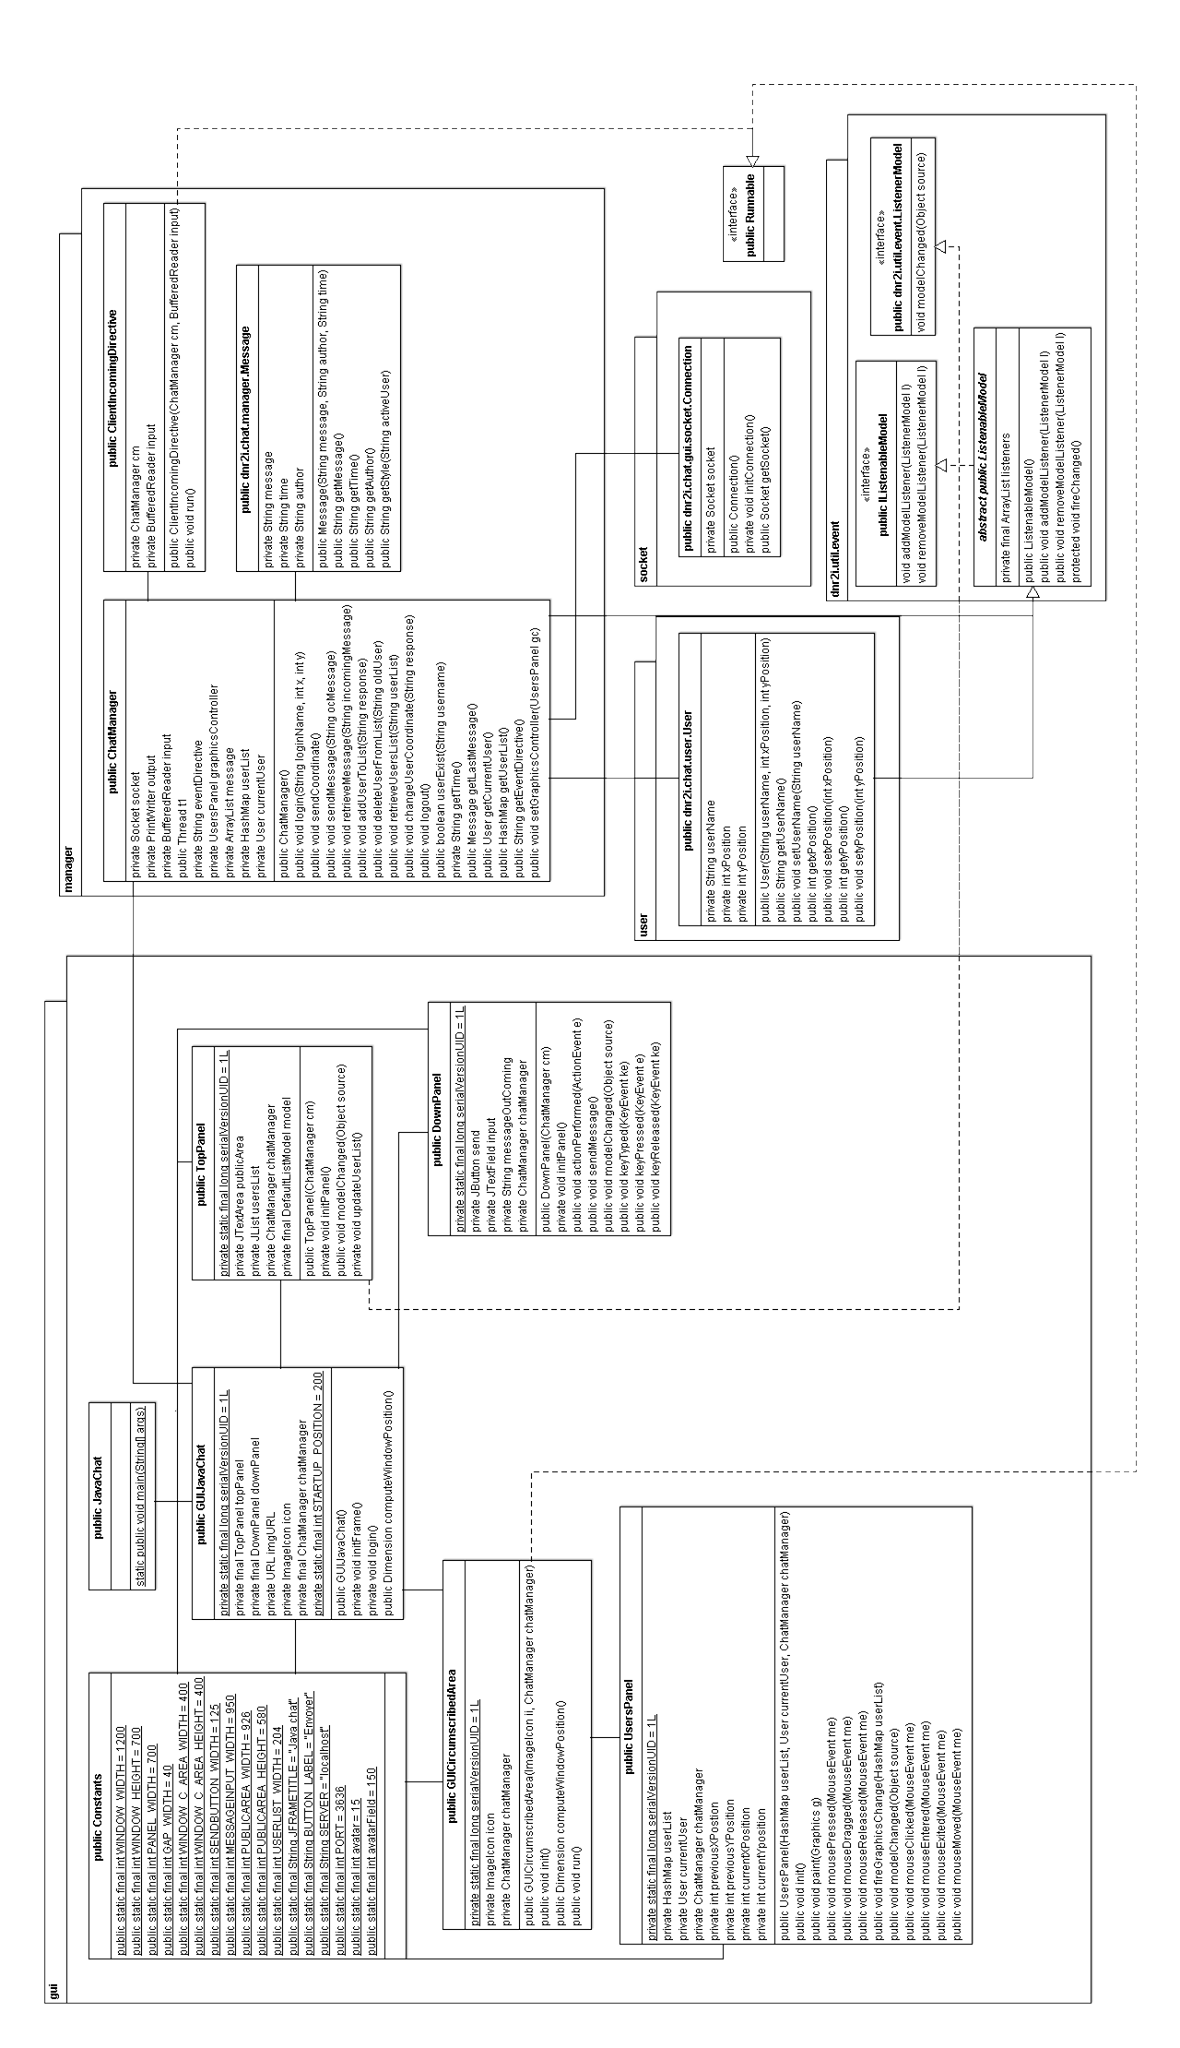
\includegraphics[height=22cm]{umlClientTurn.png}
        \caption{Uml de l'application client}
      \end{figure}
      \bigbreak

      \begin{figure}[!ht]%
        \centering 
        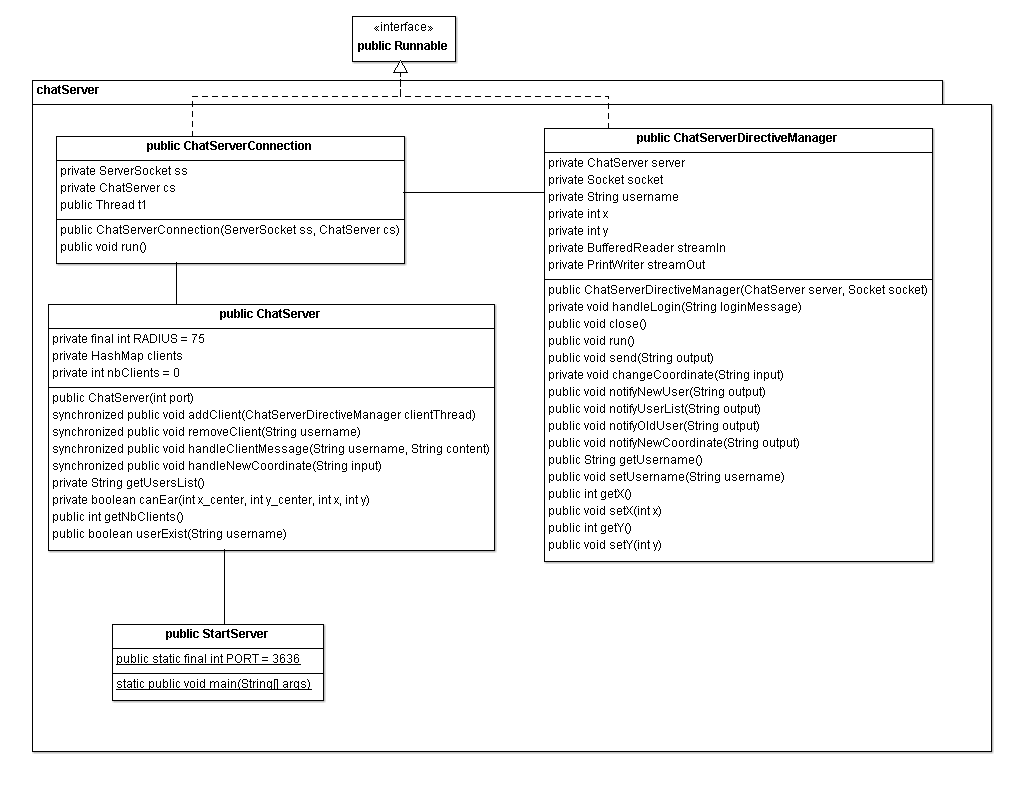
\includegraphics[width=16cm]{umlServeur.png}
        \caption{Uml de l'application serveur}
      \end{figure}

  \chapter{Interface client}

    L’interface graphique implémentée à l’aide de la librairie Swing est découpée en deux fenêtres distinctes. Une fenêtre de Chat, ainsi qu’une fenêtre de visualisation des avatars.
    \medbreak
    La fenêtre du chat est découpée de la manière suivante :
    \begin{itemize}
      \item Un Top Panel contenant une zone « Public Area » où les textes utilisateurs s’affichent et une zone « User list » indiquant les utilisateurs connectés à l’application.
      \item Un Down Panel comprenant une zone de saisie de texte et un bouton envoyer.
    \end{itemize}
    \bigbreak
    La seconde fenêtre comprend un unique Panel, User Panel contenant la liste des avatars présents sur le Chat.
    \medbreak

    \begin{figure}[!ht]%
      \centering 
      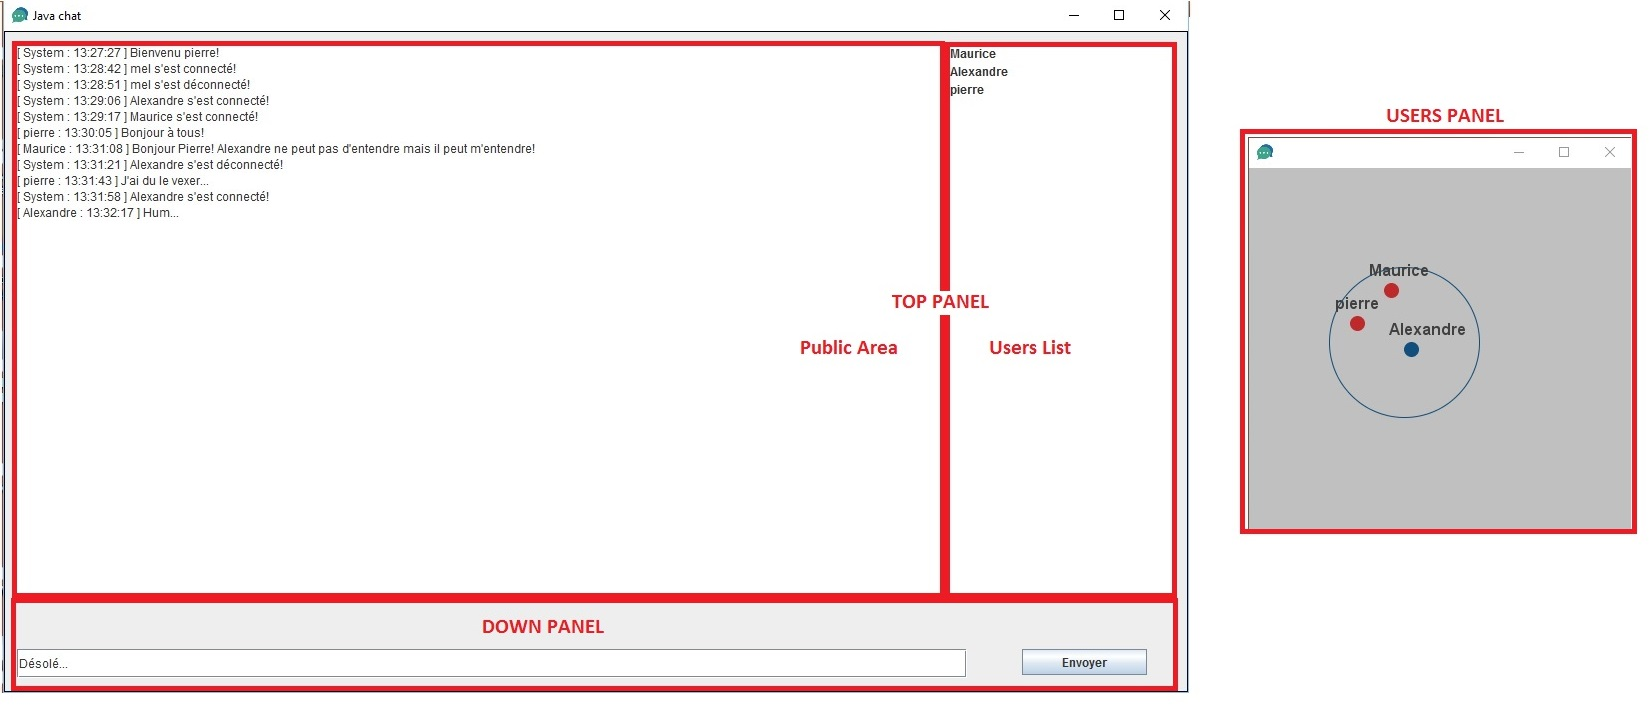
\includegraphics[width=16cm]{javaChatZonePrez.jpg}
    \end{figure}
    \bigbreak

    L’application utilisant le Pattern MVC, celle-ci comprend deux JFrame, GUIJavaChat et GUICircumscribedArea contenant l’ensemble des Panels. Ceux-ci sont instanciés prenant en paramètre le \textbf{modèle}.
    \medbreak
    Pour l’ensemble de la gestion des interactions utilisateurs, il a été nécessaire d’implémenter le \textbf{Pattern Observer}. Pour se faire le package créer en cours \emph{« dnr2i.util.event »} a été employé.

    \section{Le panel supérieur}
    Pour l’organisation du Top Panel, ainsi que pour une gestion plus précise des positionnements des éléments, nous avons utilisés un « GroupLayout ». Celui-ci, permet un placement précis de chacun des éléments à la fois horizontal et vertical, (cf figure ci-dessous).
    \medbreak
    \begin{figure}[!ht]%
      \centering 
      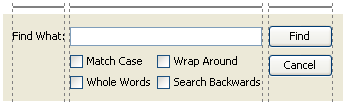
\includegraphics[width=10cm]{deecoupageGroupLayout.jpg}
      \caption{fig. découpage Group Layout (source : docs.oracle.com) }
    \end{figure}
    \bigbreak
    Dans le cadre du MVC, Ce panel étant une Vue, il implémente un ListenerModel qui a chaque changement dans le modèle, affiche d’une part les nouveaux messages (sous réserve d'appartenance à la zone circonscrite de la personne envoyant le message) et d’autre part la liste mise à jour des « T’chateurs » présent sur le serveur.

    \section{Le panel inférieur}
    Tout comme le panel supérieur, celui-ci est organisé via l’utilisation du « GroupLayout » pour les mêmes raisons qu’évoquées précédemment.
    \medbreak
    Le panel inférieur, en sus du ListenerModel, implémente un ActionListener et un KeyListener.
    \medbreak
    \begin{itemize}
      \item ActionListener permet de capter le clic sur le bouton, et de déclencher la méthode \textbf{sendMessage()};
      \item KeyListener quant à lui surveille l’entrée clavier « Entrée (KeyEvent.VK\_ENTER) » afin d’appeler la méthode d’envoi de message.
    \end{itemize}
    \bigbreak

    \section{La carte}
    L’interface de gestion des avatars se compose d’un seul Panel implémentant les interfaces ListenerModel, MouseListener, MouseMotionListener.
    \medbreak
    Pour dessiner l’ensemble des avatars, la méthode paint est redéfinie. Celle-ci a été choisie car elle offre la possibilité, en faisant appel à la méthode mère « super.paint(g) », de rafraichir chaque frame et évite les artefacts graphiques en cas de mouvement des avatars.
    \medbreak
    Pour l’affichage des avatars et pour un rendu plus fin, l’objet Graphics2D a été choisi. Celui-ci permet l’utilisation de l’anti-aliasing via la méthode : mainAvatar.setRenderingHint(RenderingHints.KEY\_ANTIALIASING,RenderingHints.VALUE\_ANTIALIAS\_ON);
    \medbreak
    L’avatar de l’utilisateur courant est dessiné via 3 composantes. Une composante \textbf{drawString} qui affiche son nom, une composante \textbf{fillOval} qui dessine son point et enfin \textbf{drawOval} qui détermine le cercle qui définit la zone circonscrite.
    \medbreak
    La position des avatars des différents T’chatteurs est mise à jour à chaque changement du modèle.
    \medbreak
    Pour mouvoir l’avatar courant, les interfaces MouseListener, et MouseMotionListener sont implémentées.
    \medbreak
    Ici, seul les méthodes mousePressed(bouton de la souris pressé), mouseDragged(souris déplacée) et mouseReleased(bouton de la souris relâché) sont redéfinies.
    \bigbreak
    \begin{itemize}
      \item mousePressed : on assigne la position courante comme position précédente.
      \item mouseDragged : on gère le mouvement de l’avatar.
      \item mouseReleased : on envoie au serveur les nouvelles coordonnées pour mise à jour.
    \end{itemize}

    \section{Les classes messages et utilisateur}
      \subsection{Classe message}
        La classe message définit ce qu’est un message. Elle est pourvue de trois attributs:
        \begin{itemize}
          \item Message : contenu d’un message utilisateur
          \item Time : heure à laquelle le message est envoyé
          \item Author : l’auteur du message
        \end{itemize}
        \bigbreak
        Elle dispose d’accesseurs associés et d’une méthode getStyle qui permet en fonction de l’utilisateur d’afficher une couleur au message (gris pour le serveur, bleu pour l’utilisateur courant et noir pour les autres T’chatteurs ). Notons que cette méthode n'est pour le moment pas utilisé car nécessiterait une transformation importante du Panel inférieur.

      \subsection{Classe utilisateur}
        La classe User définit ce qu’est un utilisateur. Celle-ci se compose de trois attributs également. Cette classe dérive de ListenableModel et ce afin d’informer tous changements au modèle via la fonction firechanged(). Elle dispose des accesseurs et mutateurs correspondants aux attributs.
        \begin{itemize}
          \item Username : son pseudonyme
          \item xPosition : sa position sur l’axe des abscisses
          \item yPosition : sa position sur l’axe des ordonnées.
        \end{itemize}

  \chapter{Le serveur}

    \begin{figure}[!ht]%
      \centering 
      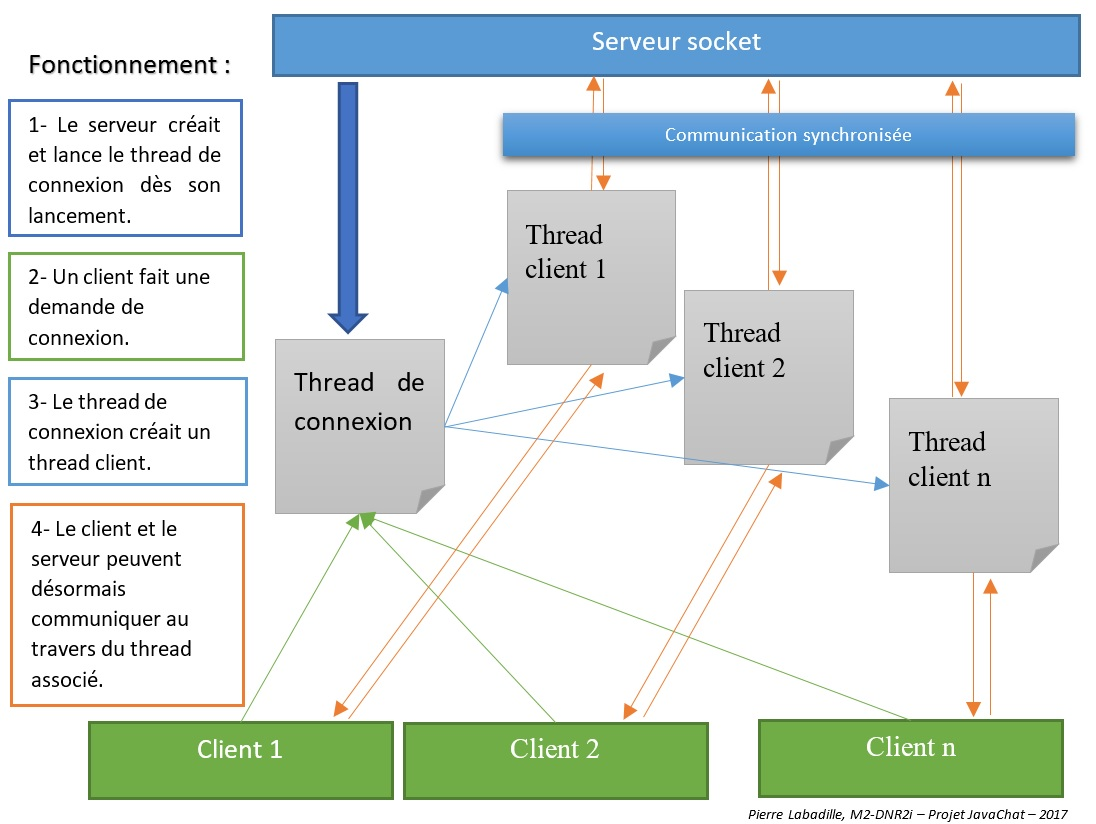
\includegraphics[width=16cm]{serverWorks.jpg}
    \end{figure}

    \bigbreak
    Le schéma ci-dessus explique comment le serveur fonctionne par étape. Chaque étape est symbolisée par une fléche de la même couleur. Il faut bien noter ici que le thread de connexion est entièrement maitrisé par le socket serveur. Ce dernier ne communique pas avec le serveur. Il va capter les directives de LOGIN envoyées par les clients et se charger de leurs créer et associer un thread.
    \medbreak
    Ce thread sera attentif aux directives entrantes de son client et pourra lui envoyer des directives serveurs. Il communique directement avec le serveur et son client associé. Il faut noter que ce thread est le seul intermédiaire entre le serveur et le client, sans lui, ils ne peuvent plus communiquer. Notons enfin la communication entre le serveur et ses threads clients est "synchronized" afin d'éviter tout conflit d'accès aux données partagées (accès concurrentiel).

    \section{Le socket serveur}
      Le socket serveur est créé avec pour seul argument le numéro de port sur lequel il devra communiquer. Dès sa création, celui-ci initialise une HashMap qui contiendra les futurs threads clients et créait un thread qui se chargera d'accepter les connexions clients.
      \medbreak
      Son rôle sera ici de choisir quelles informations envoyer à quel client (les informations seront envoyés et réceptionnées directement par le biais du thread client associé). Les threads clients feront donc appels à ses méthodes qui appeleront d'autres méthodes des threads clients concernés.
      \medbreak
      Vous trouverez dans les sous-sections ci-dessous des détails sur ses fonctionnalités principales.

      \subsection{Ajout de client}
        \say{\emph{public synchronized void addClient\(ChatServerDirectiveManager clientThread\) throws IOException}}
        \medbreak
        Cette méthode est appelée par un thread client lors de sa création. Dans un premier temps elle permet de référencer le thread dans la HashMap du socket et dans un second d'appeler les threads clients déjà présent pour les informer de la connexion d'un nouvel utilisateur.
        \medbreak
        Coté technique cette méthode est synchronized afin de gérer des potentiels accès concurentiels et utilise un itérateur pour parcourir la HashMap.

      \subsection{Supression de client}
        \say{\emph{public synchronized void removeClient(String username) throws IOException}}
        \medbreak
        Cette méthode est l'exact opposé de la méthode précédente. Elle est appelée lorsqu'une directive de déconnexion est reçue par un thread et se charge de déxindexer l'instance et de notifier les autres clients du départ de l'utilisateur.

      \subsection{Gestion de message client}
        \say{\emph{public synchronized void handleClientMessage(String username, String content)}}
        \medbreak
        Cette méthode est une des plus importante puisque c'est elle qui va déterminer quels utilisateurs pourront recevoir le message de tel autre en fonction de leurs coordonées respectives.
        \medbreak
        La zone d'écoute visible sur la carte dans l'interface utilisateur est un cercle et cette classe utilise donc une constante contenant le rayon de ce cercle (ici 75). La liste des threads utilisateurs est parcourue par le biais d'un itérateur et pour chacun d'entre eux la méthode \emph{canEar(int x\_center, int y\_center, int x, int y)} est appelée.
        \medbreak
        Cette méthode utilise un théorème de Pythagore afin de vérifier si les coordonées de l'utilisateur sont dans le cercle ou non:
        \medbreak
        \say{\emph{\textbf{(x - x\_center)² + (y - y\_center)² <= radius²} où x/y\_center représentent les coordonées de l'utilisateur qui a écrit le message.}}
        \medbreak
        L'inférieur ou égal est utilisé afin de prendre en compte tous les utilisateurs dans et sur le cercle. Utiliser '>' représenterait les personnes à l'exterieur du cercle et '==' les utilisateurs se trouvant sur sa délimitation (son tracé).

      \subsection{Gestion de changement de coordonée}
        \say{\emph{public synchronized void handleNewCoordinate(String input)}}
        \medbreak
        Cette méthode est utilisée pour prévenir le changement de coordonée d'un utilisateur à tous les autres.

      \subsection{Génération de la liste des clients connectés}
        \say{\emph{private String getUsersList()}}
        \medbreak
        Cette méthode est appelée uniquement après la création d'un nouveau thread client. Elle permet de préparer une liste contenant les informations des autres clients afin de lui retourner.

    \section{Le thread de connexion}
      Ce thread est très simple. Il attend l'arrivée de demande de connexion par le biais de .accept(). Il faut bien noter que tant qu'aucune demande de connexion n'arrive, le thread se trouve dans un etat "en attente" géré par automatiquement par ".accept()". La boucle ne tourne donc qu'une seule fois par connexion.
      \medbreak
      Lorsqu'une connexion est demandée ce thread créait un thread client associé. Toutes les futures communication auront alors lieu entre le client et son thread associé coté serveur.

    \section{Le gestionnaire de directive (thread client)}
      Dès sa construction, le thread client ouvre le buffer d'entrée et prépare celui de sortie afin de pouvoir communiquer avec le client. Il se met ensuite en attente de reception du login de l'utilisateur (et ce directement dans le constructeur). Si jamais la directive de connexion reçue n'est pas correcte, il met fin à sa construction et se ferme.
      \medbreak
      Dans le cas où la directive de connexion est correcte, il est alors ajouté à la liste des threads clients dans le serveur socket et commence à écouter les directives clients. De la même façon que le thread de connexion, "readLine()" met automatiquement en pause le thread tant qu'il ne reçoit aucune directive. 
      \medbreak
      Le serveur peut à tout moment demander au thread d'effectuer une action, généralement envoyer une information au client mais également changer ses coordonées par exemple. 
      \medbreak
      Quand le thread reçoit une directive client, il la traite par le biais d'un switch et effectue l'action correspondante. Cette action consiste généralement à appeler une ou plusieurs fonction du serveur socket qui demandera ensuite à chacun des threads clients impliqués d'envoyer la réponse appropriée à son client.

  \chapter{Interaction entre le serveur et le client}

    \section{L'interaction client-serveur}
    Chacun des protocoles envoyés au client par le serveur (et inversement) fonctionnent de la même façon. On envoit dans un premier temps le nom du protocole puis dans un second sont contenu (avec une forme normalisée). Notons qu'aucune réponse n'est attendue, dans certain cas le serveur ou le client répondent aux protocoles par un autre mais celà n'est pas considéré comme étant une réponse (mais bien un nouveau protocole).
    \bigbreak
    \underline{\textbf{Protocoles Client vers Serveur:}}
    \medbreak
    \begin{itemize}
      \item \textbf{Protocole pour connecter un client au serveur}
        \begin{itemize}
          \item Nom du protocole: "LOGIN"
          \item Forme du contenu envoyé: USERNAME</END>X\_POSITION</END>Y\_POSITION
          \item Réaction du serveur:
            \begin{itemize}
              \item Le serveur créait un nouveau thread associé au client.
              \item Un protocole "SET\_USERS\_LIST" est envoyé au client venant de se connecter
              \item Un protocole "SET\_NEW\_USER" est envoyé à tous les autres clients.
            \end{itemize}
        \end{itemize}
      \item \textbf{Protocole pour envoyer un nouveau message au serveur}
        \begin{itemize}
          \item Nom du protocole: "SET\_MSG"
          \item Forme du contenu envoyé: USERNAME</END>MESSAGE</END>TIME
          \item Réaction du serveur: un protocole "GET\_MSG" est envoyé à tous les clients éligibles.
        \end{itemize}
      \item \textbf{Protocole pour mettre à jour ses coordonées suite à un déplacement}
        \begin{itemize}
          \item Nom du protocole: "SET\_COORDINATE"
          \item Forme du contenu envoyé: USERNAME</END>X\_POSITION</END>Y\_POSITION
          \item Réaction du serveur: un protocole "SET\_NEW\_COORDINATE" est envoyé à tous les clients exceptés celui-ci et mise à jour des coordonées de l'utilisateur au niveau du serveur.
        \end{itemize}
      \item \textbf{Protocole pour déconnecter un client du serveur}
        \begin{itemize}
          \item Nom du protocole: "LOGOUT"
          \item Forme du contenu envoyé: USERNAME
          \item Réaction du serveur: le thread associé au client est détruit et un protocole "SET\_OLD\_USER" est envoyé à tous les autres clients.
        \end{itemize}
    \end{itemize}

    \bigbreak
    \underline{\textbf{Protocoles Serveur vers Client(s):}}
    \medbreak
    \begin{itemize}
      \item \textbf{Protocole pour envoyer la liste des clients connectés à un client venant de se connecter}
        \begin{itemize}
          \item Nom du protocole: "SET\_USERS\_LIST"
          \item Forme du contenu envoyé: USERNAME</END>X\_POSITION</END>Y\_POSITION</USER> * n user.
          \item Réaction du client: ajout des nouveaux utilisateurs et mise à jour de la vue et de la vue graphique.
        \end{itemize}
      \item \textbf{Protocole pour informer qu'un nouvel utilisateur vient de se connecter}
        \begin{itemize}
          \item Nom du protocole: "SET\_NEW\_USER"
          \item Forme du contenu envoyé: USERNAME</END>X\_POSITION</END>Y\_POSITION
          \item Réaction du client: ajout du nouvel utilisateur et mise à jour de la vue.
        \end{itemize}
      \item \textbf{Protocole pour distribuer un message aux clients éligibles}
        \begin{itemize}
          \item Nom du protocole: "GET\_MSG"
          \item Forme du contenu envoyé: USERNAME</END>MESSAGE</END>TIME
          \item Réaction du client: création de la nouvelle instance de message et mise à jour de la vue.
        \end{itemize}
      \item \textbf{Protocole pour informer du changement de position d'un utilisateur}
        \begin{itemize}
          \item Nom du protocole: "SET\_NEW\_COORDINATE"
          \item Forme du contenu envoyé: USERNAME</END>X\_POSITION</END>Y\_POSITION
          \item Réaction du client: mise à jour des coordonées de l'utilisateur concerné et mise à jour de la vue graphique.
        \end{itemize}
      \item \textbf{Protocole pour informer qu'un utilisateur vient de se déconnecter}
        \begin{itemize}
          \item Nom du protocole: "SET\_OLD\_USER"
          \item Forme du contenu envoyé: USERNAME
          \item Réaction du client: destruction de l'instance utilisateur correspondante et mise à jour de la vue et de la vue graphique.
        \end{itemize}
    \end{itemize}

    \section{Le manager client}
      Le manager client (\emph{ChatManager}) est le cerveau de l'application client. Il fonctionne de façon similaire au socket serveur: lors de sa création il construit une instance de connexion afin de réccupèrer le socket de communication avec le serveur. Il va ensuite ouvrir ses buffers de lecture et d'écriture et constuire un thread qui aura pour objectif d'attendre des directives serveurs.
      \medbreak
      Tout envoit de directive au serveur est directement géré dans cette classe. Elle n'utilise néanmoins jamais son buffer de lecture qui est délégué à son thread "ClientIncomingDirective".
      \medbreak
      Notons enfin que cette classe "fire" deux types de changement, le traditionnel "\textbf{fireChanged()}" qui est utilisé pour mettre à jour la vue (message, liste des utilisateurs...) mais également une méthode "\textbf{fireGraphicsChange()}" afin d'actualiser la carte.

    \section{Le thread client de gestion des directives}
      Cette classe (\emph{ClientIncomingDirective}) va uniquement servir à recevoir et interpréter les directives envoyées par le serveur. Elle fonctionne par le biais d'un "\textbf{readLine()}" permettant de mettre en pause le thread automatiquement quand aucune donnée n'est transmise et d'appliquer la méthode associée à une directive dans le manager client. Cette interprétation des directives ce fait très simplement par le biais d'un switch.
      \medbreak
      Il faut enfin noter que cette classe n'est pas capable d'envoyer des directives au serveur, elle se contente uniquement de les recevoir.

  \chapter{Conclusion}

    \section{Difficultés rencontrées}
      La compréhension du système de socket et de thread, bien qu'explicité en cours, n'a pas été évident. La logique de leurs fonctionnements est inhabituels et il a fallut bien la comprendre avant de réussir à l'utiliser correctement.
      \medbreak
      Le manque de temps et de sommeil induit pas ces dernières semaines très chargées en projet sur des technologies et langages totalement différents.

    \section{Apport personnel}
      Tout d'abord nous somme heureux d'avoir pu développer une application executable et visuelle hors console.
      \medbreak
      Nous avons acquéris de nouvelles compétences concernant la logique serveur, les threads et les interfaces graphiques en Java.
      \medbreak
      En sus des nouvelles compétences acquises,  cela nous a permis de contempler de nouvelles perspectives quand à ce qu'on peut espérer réaliser  avec java, en particulier avec les librairies graphiques.
      \medbreak
      Et comme d'habitude, ce fut un plaisir certain de travailler en groupe, en particulier dans celui-ci qui à partagé la même motivation, implication et cohérence.

\end{document}
